\let\negmedspace\undefined
\let\negthickspace\undefined
\documentclass[journal]{IEEEtran}
\usepackage[a5paper, margin=10mm, onecolumn]{geometry}
\usepackage{lmodern} 
\usepackage{tfrupee} 

\setlength{\headheight}{1cm} % Set the height of the header box
\setlength{\headsep}{0mm}     % Set the distance between the header box and the top of the text

\usepackage{gvv-book}
\usepackage{gvv}
\usepackage{cite}
\usepackage{amsmath,amssymb,amsfonts,amsthm}
\usepackage{algorithmic}
\usepackage{graphicx}
\usepackage{textcomp}
\usepackage{xcolor}
\usepackage{txfonts}
\usepackage{listings}
\usepackage{enumitem}
\usepackage{mathtools}
\usepackage{gensymb}
\usepackage{comment}
\usepackage[breaklinks=true]{hyperref}
\usepackage{tkz-euclide} 
\usepackage{listings}                                      
\def\inputGnumericTable{}                                 
\usepackage[latin1]{inputenc}                                
\usepackage{color}                                            
\usepackage{array}                                            
\usepackage{longtable}
\usepackage{multicol}
\usepackage{calc}                                             
\usepackage{multirow}                                         
\usepackage{hhline}                                           
\usepackage{ifthen}                                           
\usepackage{lscape}
\begin{document}

\bibliographystyle{IEEEtran}
\vspace{3cm}

\title{5.8.29}
\author {EE25BTECH11031 - Sai Sreevallabh}
% \maketitle
% \newpage
% \bigskip
{\let\newpage\relax\maketitle}

\renewcommand{\thefigure}{\theenumi}
\renewcommand{\thetable}{\theenumi}
\setlength{\intextsep}{10pt} % Space between text and floats


\numberwithin{equation}{enumi}
\numberwithin{figure}{enumi}
\renewcommand{\thetable}{\theenumi}

\textbf{Question: }\\

 $2$ women and $5$ men can together finish an embroidery work in $4$ days, while $3$ women and $6$ men can finish it in $3$ days. Find the time taken by $1$ women alone to finish the work, and also that taken by $1$ man alone.\\

\textbf{Solution: }\\ 

Let the fraction of work done by a woman in a day be $x$ and the fraction of work done by a man in a day be $y$, represented as 
\begin{align}
    \vec{x} = \myvec{x\\y}
\end{align}

Also, if $a$ days are taken for a work to complete, the fraction of work completed in a single day is $\frac{1}{a}$.

% Then the number of days taken by the woman and the man would respectively be $\frac{1}{a}$ and $\frac{1}{b}$. 

Using the above, we can write the given data into two equations:

\begin{align}
    \myvec{2&5}\vec{x} = \frac{1}{4} \label{eq2}
\end{align}

\begin{align}
    \myvec{3&6}\vec{x} = \frac{1}{3} \label{eq3}
\end{align}

Converting into Reduced Row Echelon Form:

\begin{align}
    \augvec{2}{1}{2&5&\frac{1}{4}\\[1ex]3&6&\frac{1}{3}}
    \xleftrightarrow[]{R_1\xrightarrow{}\frac{1}{2}R_1} 
    \augvec{2}{1}{1&\frac{5}{2}&\frac{1}{4}\\[1ex]3&6&\frac{1}{3}}
\end{align}

\begin{align}
    \augvec{2}{1}{1&\frac{5}{2}&\frac{1}{4}\\[1ex]3&6&\frac{1}{3}}
    \xleftrightarrow[]{R_2\xrightarrow{}R_2-3R_1}
    \augvec{2}{1}{1&\frac{5}{2}&\frac{1}{4}\\[1ex]0&-\frac{3}{2}&-\frac{1}{24}}
\end{align}

\begin{align}
    \augvec{2}{1}{1&\frac{5}{2}&\frac{1}{4}\\[1ex]0&-\frac{3}{2}&-\frac{1}{24}}
    \xleftrightarrow[]{R_2\xrightarrow{}-\frac{2}{3}R_2}
    \augvec{2}{1}{1&\frac{5}{2}&\frac{1}{4}\\[1ex]0&1&\frac{1}{36}}
\end{align}

\begin{align}
    \augvec{2}{1}{1&\frac{5}{2}&\frac{1}{4}\\[1ex]0&1&\frac{1}{36}}
    \xleftrightarrow[]{R_1\xrightarrow{}R_1-\frac{5}{2}R_2}
    \augvec{2}{1}{1&0&\frac{1}{18}\\[1ex]0&1&\frac{1}{36}}
\end{align}

We get
\begin{align}
    \vec{x} = \myvec{\frac{1}{18}\\[1ex]\frac{1}{36}}
\end{align}\\

The number of days can be written as
\begin{align}
    \frac{1}{y} = 36 \ \  \text{and} \ \ \frac{1}{x} = 18
\end{align}\\

$\therefore$ The time taken by one woman alone to finish the work is $18$ days, and the time taken by one man alone to finish the work is $36$ days.\\



(The below graph represents the solution to the equations \eqref{eq2} and \eqref{eq3})

\begin{figure}[h]
    \centering
    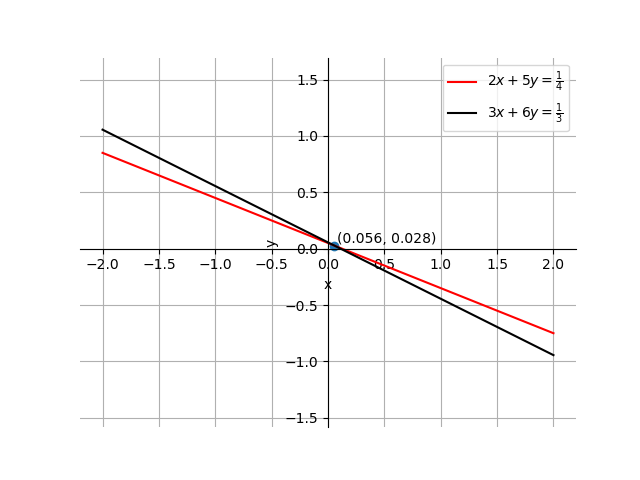
\includegraphics[width=1\columnwidth]{Figs/plot(py).png}
\end{figure}

\end{document}
